\chapter{Seitenlayout}

In diesem Kapitel treten wir einen Schritt zurück und betrachten die zu
gestaltende Seite als Ganzes. Anders ausgedrückt: Nach der
Mikrotypographie wenden wir uns nun der \emph{Makrotypographie} zu. Hier geht es also um
die Frage wo auf einer Seite Textelemente platziert werden können – stets mit
dem Ziel, einerseits ein harmonisches und »ruhiges« Gesamtbild zu erzeugen und
andererseits die Lesbarkeit an sich zu optimieren.

Wir beginnen konservativ und studieren zunächst die strengen und weitestgehend
standardisierten Prinzipien des Buchsatzes. Viele dieser Prinzipien lassen sich
auf andere Formate übertragen; wir geben am Ende dieses Kapitels einen Ausblick
dazu.

\section{Satzspiegel}

Als \emph{Satzspiegel} wird der Bereich der Seite bezeichnet, auf dem der
eigentliche Text (siehe unten für Kopf- und Fußzeilen) stehen kann. Er wird
begrenzt durch die vier Seitenränder. Ziel ist es, den Satzspiegel so zu wählen,
dass er »harmonisch« wirkt.

\subsection{Klassische Buchdoppelseite}

Wir wollen dies zunächst am klassischen Beispiel eines Buches beschreiben. Ist
ein Buch aufgeschlagen, so sieht man eine \emph{linke} und eine \emph{rechte}
Seite. Da beiden Satzspiegel zueinander »am Buchsteg gespiegelt« ausgerichtet
sein sollen, ist es daher sinnvoll, die Seitenränder »oben«, »unten«, »innen«
und »außen« zu betrachten. Im strengen klassischen Buchsatz gelten folgende
Prinzipien:
\begin{enumerate}
\item Der äußere Rand ist doppelt so groß wie der innere.
\item Der untere Rand ist doppelt so groß wie der obere.
\item Das Seitenverhältnis des Satzspiegels gleicht dem der Seite.
\end{enumerate}
Eine Umformulierung der vielleicht etwas willkürlich wirkenden ersten Regel ist,
dass der \emph{gemeinsame} innere Rand genauso groß wie jeder der äußeren Ränder
ist. Befolgt man all diese Regeln, bleibt nur noch ein Freiheitsgrad übrig, und
dieser kann beschrieben werden durch das Breitenverhältnis zwischen Satzspiegel
und Seite. In \cref{fig:Satzspiegel} finden sich zwei Beispiele, wo dieses
Verhältnis einmal 70\,\% und einmal 60\,\% beträgt.

\begin{figure}
  \centering
  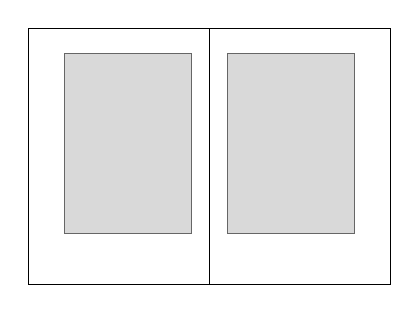
\begin{tikzpicture}[scale=2.3]
    \draw (0,0) rectangle (2,1.414);
    \draw (1,0) -- (1,1.414);
    \draw[black!60,thin,fill=black!15] (.2,.282) rectangle (.9,1.273);
    \draw[black!60,thin,fill=black!15] (1.1,.282) rectangle (1.8,1.273);
  \end{tikzpicture}\quad
  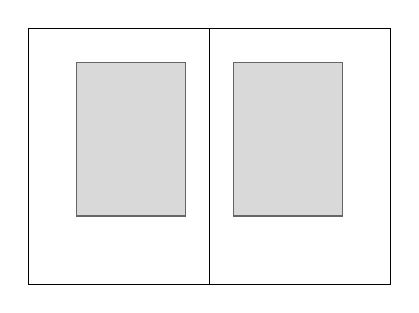
\begin{tikzpicture}[scale=2.3]
    \draw (0,0) rectangle (2,1.414);
    \draw (1,0) -- (1,1.414);
    \draw[black!60,thin,fill=black!15] (.267,.377) rectangle (.867,1.226);
    \draw[black!60,thin,fill=black!15] (1.133,.377) rectangle (1.733,1.226);
  \end{tikzpicture}
  \caption{Zwei Satzspiegel, die den klassischen Prinzipien genügen. Die
    Ausgangsseite hat (wie alle \acr{DIN}-Formate) ein Seitenverhältnis von
    1\,:\,$\sqrt{\text{2}}$. Das Breitenverhältnis zwischen Satzspiegel und Seite ist
    einmal 70\,\% (links) und einmal 60\,\% (rechts).}
  \label{fig:Satzspiegel}
\end{figure}

\subsection{Rasterteilung}

Anstatt dieses Breitenverhältnis anzugeben, wird in der Praxis der Satzspiegel
häufig durch \emph{Rasterteilung} bestimmt: Wir fixieren eine natürliche Zahl
$n$ und unterteilen die Seite gleichmäßig in $n$ Spalten und $n$ Zeilen. Nun
nehmen wir innen eine Spalte, außen zwei Spalten, oben eine Zeile und unten zwei
Zeilen weg; der verbleibende Bereich ist der Satzspiegel, siehe
\cref{fig:DIV}. Wir nennen $n$ den \emph{Rasterfaktor}. Auf diese
Weise sind nur noch Breitenverhältnisse der Form $\frac{n-3}{n}$ möglich. In
\LaTeX\ nimmt die \acr{KOMA}-Klasse \verb!scrbook! automatisch eine
Rasterteilung vor. Der Rasterfaktor kann z.\,B. durch \verb!DIV=9!
festgesetzt werden.

\begin{figure}
  \centering
  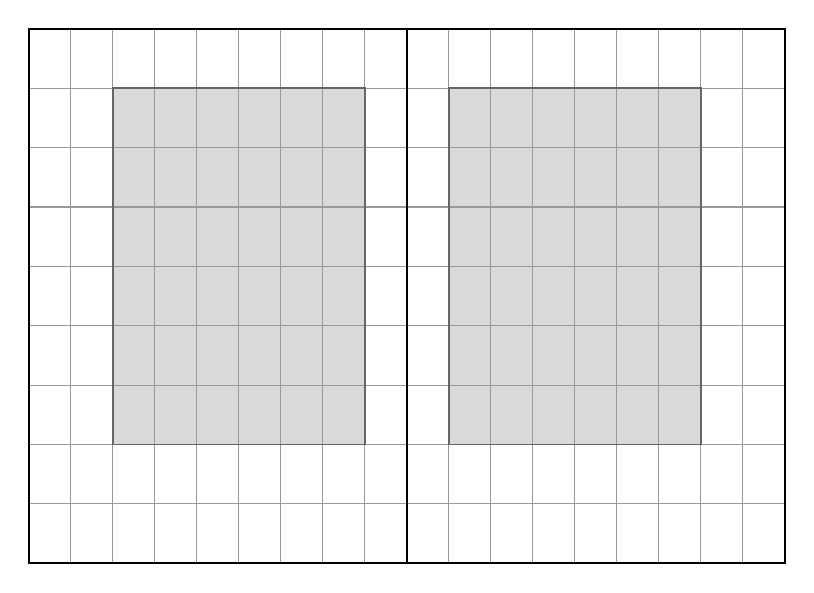
\begin{tikzpicture}[scale=4.8]
    \fill[black!15] ({2/9},{2*sqrt(2)/9}) rectangle ({8/9},{8*sqrt(2)/9});
    \fill[black!15] ({2-(2/9)},{2*sqrt(2)/9}) rectangle ({2-(8/9)},{8*sqrt(2)/9});
    \foreach \i in {1,...,8}{
      \draw[thin,black!40] ({\i/9},0) -- ({\i/9},{sqrt(2)});
      \draw[thin,black!40] (0,{\i*sqrt(2)/9}) -- (2,{\i*sqrt(2)/9});
      \draw[thin,black!40] ({(9+\i)/9},0) -- ({(9+\i)/9},{sqrt(2)});
    };
    \draw[semithick,black!60] (2/9,{2/9*sqrt(2)}) rectangle ({8/9},{8/9*sqrt(2)});
    \draw[semithick,black!60] (10/9,{2/9*sqrt(2)}) rectangle ({16/9},{8/9*sqrt(2)});
    \draw[thick] (0,0) rectangle (2,{sqrt(2)});
    \draw[thick] (1,0) -- (1,{sqrt(2)});
  \end{tikzpicture}
  \caption{Eine Rasterteilung mit Rasterfaktor 9, auch
    \emph{Neunerteilung} genannt. Das entstehende Breitenverhältnis ist
    \smallfrac69\,=\,\smallfrac23.}
  \label{fig:DIV}
\end{figure}


\subsection{Bindekorrektur}

Soll das Dokument als Buch gebunden werden, so kann innen etwas Platz durch die
Bindung verloren gehen, sodass bei einer aufgeschlagenen Seite der gemeinsame
innere Rand \emph{kleiner} als jeder der äußeren Ränder ist. Dem wird durch die
sogenannte \emph{Bindekorrektur} entgegengewirkt: Hierbei wird von der Seite
innen ein Streifen fester Breite (z.\,B. 5\,mm) ignoriert und dann nur noch der
übrige Bereich einer Rasterteilung unterzogen. Der erforderliche Wert hängt von
der Bindungsart ab und ist von der Binderei zu erfragen. Ist er bekannt, kann er
leicht z.\,B. durch \verb!BCOR=5mm! eingestellt werden.

\subsection{Einseitiges Layout}

Im einseitigen Layout (geeignet für Dokumente, die nicht wie ein Buch
»aufgeklappt« werden) sind die Seitenränder links und rechts gleich groß; die
übrigen beiden Prinzipien gelten unverändert. Nicht ganz korrekterweise wird
auch hier der Begriff der \emph{Rasterteilung} verwendet, im Gegensatz zu obiger
Konstruktion werden allerdings nun links und rechts 1,5 Spalten entfernt, siehe
\cref{fig:einseitig}. So wird zum Beispiel von der \acr{KOMA}-Klasse
\verb!scrartcl! der Satzspiegel bestimmt.

\begin{figure}
  \centering
  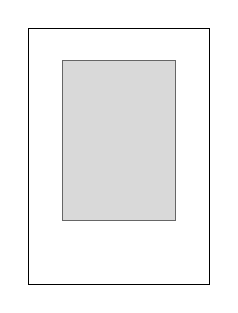
\begin{tikzpicture}[scale=2.3]
    \draw (0,0) rectangle (1,{sqrt(2)});
    \draw[black!60,thin,fill=black!15] (.1875,{.25*sqrt(2)}) rectangle (.8125,{.875*sqrt(2)});
  \end{tikzpicture}\quad
  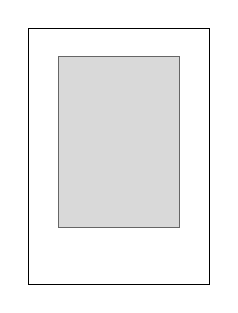
\begin{tikzpicture}[scale=2.3]
    \draw (0,0) rectangle (1,{sqrt(2)});
    \draw[black!60,thin,fill=black!15] (.167,{.222*sqrt(2)}) rectangle (.833,{.888*sqrt(2)});
  \end{tikzpicture}\quad
  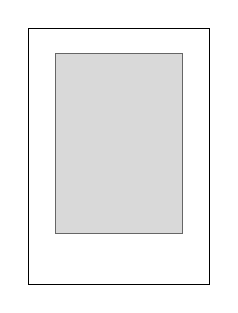
\begin{tikzpicture}[scale=2.3]
    \draw (0,0) rectangle (1,{sqrt(2)});
    \draw[black!60,thin,fill=black!15] (.15,{.2*sqrt(2)}) rectangle (.85,{.9*sqrt(2)});
  \end{tikzpicture}
  \caption{Mehrere einseitige Satzspiegel durch Rasterteilung, mit
    Rasterfaktoren 8, 9 und 10}
  \label{fig:einseitig}
\end{figure}

\subsection{Mehr Freiheit}
\label{subsec:Freiheit}

In moderneren Büchern wird das dritte Prinzip oft außer Acht gelassen. So ist
zum Beispiel dieses Skript für \acr{DIN-A5}-Papier gesetzt, d.\,h. die Seite hat
ein Verhältnis von 1\,:\,$\sqrt{\text{2}}$, während der Satzspiegel ein
Verhältnis von 3\,:\,5 hat. Ein Grund für diese Entwicklung ist vermutlich, dass
der untere Rand für zu groß befunden wurde.

\section{Zeilenlängen \emph{\&} Papierformate}

Nun stellt sich natürlich die Frage, nach welchen Kriterien das
Breitenverhältnis (bzw. der Rasterfaktor, der es am besten approximiert) gewählt
wird. Wieso nicht einfach 100\,\% (bzw. ein möglichst großer Rasterfaktor)? Die
entscheidende Einschränkung ist die \emph{Zeilenlänge}, die dadurch
quantifiziert wird, wie viele Zeichen des regulär formatierten Textes
durchschnittlich in eine Zeile passen. Konservative Typograph:innen empfehlen,
dass dieser Wert zwischen 60 und 80 Zeichen pro Zeile liegt, da ansonsten die
Lesbarkeit beeinträchtigt ist. Dieses Skript hat etwa 65 Zeichen pro Zeile. Je
nach Textgattung (etwa bei signifikantem Formelanteil) ist aber auch ein
größerer Wert geeignet. Wir weisen darauf hin, dass die Zeilenlänge von der
Laufweite der Schriftart abhängt.

Andererseits sollte natürlich auch noch ein relevanter Teil der Seite
beschreibbar sein. So sorgt ein Rasterfaktor von 7 zwar für kurze Zeilen,
allerdings wird am Ende auch nur \smallfrac{16}{49}, also etwa 32,6\,\% der
Seite bedruckt. Aus diesem Grund ist das Standardpapierformat \acr{DIN A4}
(210\,×\,297\,mm²) für die meisten Schriftstücke eigentlich zu groß, wie
\cref{tab:Papier} zeigt. Alternativen sind \acr{DIN B5} (176\,×\,250\,mm²) oder
\acr{DIN A5} (148\,×\,210\,mm²). Auf \acr{DIN A4} bietet sich hingegen ein
zwei- oder dreispaltiger Satz an.

\begin{table}
  \centering
  \begin{tabular}{rrrrr}
    \toprule
    \tableHead{Faktor} & \tableHead{Anteil} & \tableHead{DIN A4} & \tableHead{DIN B5} & \tableHead{DIN A5}\\
    \midrule
    \tab{11} & \tab{52,9}\,\% & \tab{100} & \tab{83} & \tab{72}\\
    \tab{10} & \tab{49,0}\,\% & \tab{96} & \tab{78} & \tab{68}\\
    \tab{9} & \tab{44,4}\,\% & \tab{90} & \tab{74} & \tab{64}\\
    \tab{8} & \tab{39,0}\,\% & \tab{85} & \tab{71} & \tab{61}\\
    \tab{7} & \tab{32,6}\,\% & \tab{77} & \tab{66} & \tab{57}\\
    \bottomrule
  \end{tabular}
  \caption{Anteil am Flächeninhalt und Zeilenlängen (für \acr{DIN A4}, \acr{DIN
      B5} und \acr{DIN A5}) für unterschiedliche Rasterfaktoren. Für diese
    Werte wurde die Schriftart Minion mit 11\,pt verwendet. Bei strenger
    Auslegung würde bei \acr{DIN A4} kein Rasterfaktor über 7 infrage kommen.}
  \label{tab:Papier}
\end{table}

\section{Die Stege}

Die Bereiche außerhalb des Satzspiegels nennt man auch \emph{Stege}: Es gibt
also \emph{Innen-}, \emph{Außen-}, \emph{Kopf-} und \emph{Fußsteg}. Diese Stege
können auch mit speziellem Inhalt bedruckt werden. Zwar ist der Innensteg meist
zu schmal, der Außensteg eignet sich aber gut für Randnotizen, sogenannte
\emph{Marginalien}. In diesem Skript finden sich zum Beispiel in \cref{ch:Emph}
welche. Ein Vorteil der in \cref{subsec:Freiheit} erwähnten Praxis, für den
Satzspiegel ein schmaleres Seitenverhältnis zu verwenden, ist, dass auf diese
Weise ein größerer Außensteg und somit mehr Platz für Marginalien entsteht.
Auch Kapitelnummern können auf dem Außensteg platziert werden; so ist der Beginn
eines neuen Kapitels beim Durchblättern leicht erkennbar. Zwischen Satzspiegel
und den Marginalien sollte ein horizontaler Abstand von wenigstens 1,5 Geviert
freigelassen werden.

Kopf- und Fußsteg sind, wie der Name schon vermuten lässt, ein guter Ort für
\emph{Kopf-} und \emph{Fußzeilen}. Bei Verwendung der \acr{KOMA}-Klassen in
\LaTeX\ konfiguriert man diese am einfachsten mit dem Paket
\verb!scrlayer-scrpage!. Grundsätzlich sind beide Zeilen optional, beide
\emph{können} innen, mittig und außen Inhalt tragen. Der Abstand dieser Zeilen
zum eigentlichen Satzspiegel sollte wenigstens eine Leerzeile für den Kopf und
zwei Leerzeilen für den Fuß betragen; je nachdem, wie hoch der Fußsteg ist kommt
auch ein größerer Abstand in Betracht. Während die Fußzeile meist außen
die Seitenzahl führt und ansonsten leer ist, kann die Kopfzeile auch einen
\emph{lebenden Kolumnentitel}, also z.\,B. den aktuellen Kapitelnamen,
enthalten.\looseness-1

In \cref{fig:Stege} sind die in diesem Abschnitt erwähnten Gestaltungselemente
noch einmal schematisch visualisiert.

\begin{figure}
  \centering
  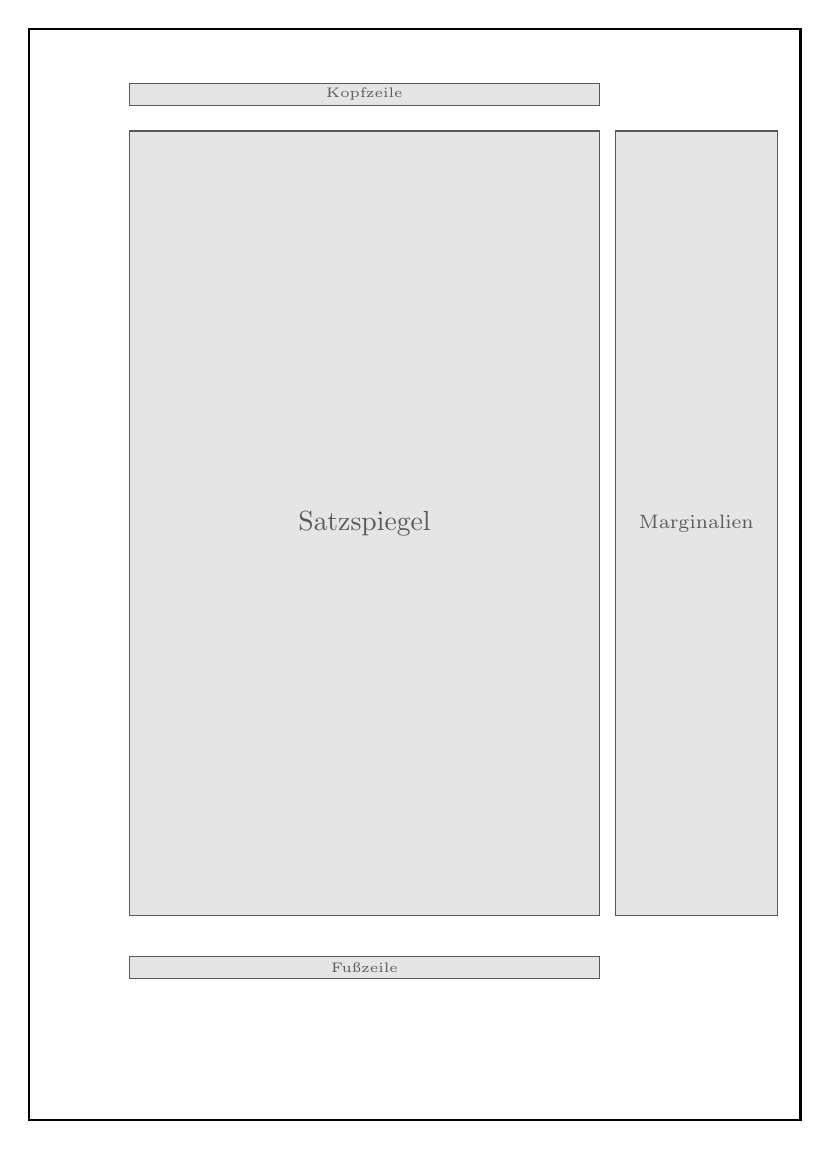
\begin{tikzpicture}[scale=9.8]
    \draw[thick] (0,0) rectangle (1,{sqrt(2)});
    \draw[black!65,thin,fill=black!10] (.13,{.1874*sqrt(2)}) rectangle (.74,{.9063*sqrt(2)});
    \draw[black!65,thin,fill=black!10] (.76,{.1874*sqrt(2)}) rectangle (.97,{.9063*sqrt(2)});
    \draw[black!65,thin,fill=black!10] (.13,{.93*sqrt(2)}) rectangle (.74,{.95*sqrt(2)});
    \draw[black!65,thin,fill=black!10] (.13,{.15*sqrt(2)}) rectangle (.74,{.13*sqrt(2)});
    \node[black!65] at (.435,{.94*sqrt(2)}) {\tiny Kopfzeile};
    \node[black!65] at (.435,{.54685*sqrt(2)}) {Satzspiegel};
    \node[black!65] at (.435,{.14*sqrt(2)}) {\tiny Fußzeile};
    \node[black!65] at (.865,{.54685*sqrt(2)}) {\scriptsize Marginalien};
  \end{tikzpicture}
  \caption{Eine rechte Buchseite mit Kopf- und Fußzeile sowie markiertem Bereich
    für Marginalien. Hier hat die Seite wieder ein Verhältnis von
    1\,:\,$\sqrt{\text{2}}$ und der Satzspiegel eines von 3\,:\,5.}
  \label{fig:Stege}
\end{figure}

\section{Umbrüche \emph{\&} Absätze}

\subsection{Zeilenumbrüche und Blocksatz}
\label{subsec:Blocksatz}

Ist eine Zeile voll, muss in der nächsten Zeile weitergeschrieben werden; es ist
also ein \emph{Zeilenumbruch} vonnöten. Umgebrochen werden kann am Ende eines
Wortes oder auch innerhalb eines Wortes zwischen zwei Silben; dann ist ein
Trennstrich (siehe \cref{subsec:Viertel}) vonnöten. Auf diese Weise passiert es
aber, dass Zeilen je nachdem, welchen Text sie enthalten, etwas zu kurz
sind. Beim im Buchsatz üblichen \emph{Blocksatz} werden darauf"|hin die
Leerzeichen (und ein kleines bisschen auch die Buchstabenzwischenräume)
gestreckt, sodass alle Zeilen bündig am rechten Ende des Satzspiegels enden. In
geringem Maße ist auch das Gegenteil möglich: Nämlich dass bei einer minimal zu
langen Zeile Leerzeichen und Zwischenräume gestaucht werden, um die Bündigkeit
zu erzielen.

Dabei ist zu beachten, dass sich Blocksatz und Silbentrennung gegenseitig
bedingen: Blocksatz ohne Silbentrennung führt rasch zu unverhältnismäßig
gestreckten Zeilen; Silbentrennung ohne Blocksatz – probiert es ruhig mal selbst
aus und bildet Euch ein Urteil.

Da es wie gesagt im Einzelfall günstiger sein kann, ein paar wenige Zeichen in
eine eigentlich schon volle Zeile zu »quetschen«, stellen Zeilenumbrüche ein
nicht-triviales Optimierungsproblem da. Für dieses nutzt man in \LaTeX\ am
besten das \verb!microtype!-Paket. Um Silben erfolgreich zu trennen, ist es
wichtig, dass über das \verb!babel!-Paket die richtige Sprache eingestellt ist.
Mit dieser Konfiguration wird das Ergebnis solide aussehen; trotzdem kann es
aber im Einzelfall nötig sein, das Ergebnis anzupassen – am einfachsten durch
minimalinvasive Umformulierungen des Textes. Manchmal muss man \LaTeX\ auch
beibringen, dass ein Wort an einer bestimmten Stelle getrennt werden darf, dies
geschieht z.\,B. durch \verb!Fak\-tor!.

\subsection{Absätze}

Ist ein Sinnabschnitt zuende, möchte man einen neuen \emph{Absatz}
beginnen. Vorweg: Dies geschieht in \LaTeX\ \emph{nicht}, indem man \verb!\\!
eingibt, sondern indem man eine Leerzeile im Quellcode (also zweimal
\keys{\return} drücken) erzeugt. Dann kann \LaTeX\ nämlich das Gewünschte tun.

Gewünscht sein können, je nach Tradition, zwei verschiedene Dinge, wobei man
sich global für eines davon entscheiden sollte: In europäischer Typographie ist
es üblich, dass der neue Absatz ohne zusätzlichen vertikalen Zwischenraum in der
nächsten Zeile beginnt, diese neue Zeile allerdings mit einem \emph{Einzug},
also einem Leerraum, von etwa einem Geviert beginnt. In \acr{US}-amerikanischer
Typographie, in der Webtypographie und zum Teil auch zunehmend in deutschen
Geschäftsbriefen ist es hingegen üblich, statt des Einzuges die beiden Absätze
durch eine \emph{Leerzeile} zu trennen.

Ein Umbruch, auf den weder ein Einzug noch eine Leerzeile folgt, ist kein
gültiger Absatz.  Ebenso ist aber auch eine Kombination aus Einzug und Leerzeile
unüblich – eine Ausnahme bildet die künstliche Streckung, um Seiten unten bündig
enden zu lassen, wie wir im nächsten Abschnitt erklären werden.

Abschließend: Die letzte Zeile eines Absatzes sollte zu wenigstens einem Drittel
der Zeilenlänge gefüllt sein.

\subsection{Seitenumbrüche}

Passt auf eine Seite keine neue Zeile mehr, muss eine neue begonnen werden; es
ist also ein \emph{Seitenumbruch} vonnöten. So weit, so gut, allerdings sollten
für ein optisch ansprechendes Ergebnis weitere Einschränkungen betrachtet
werden:
\begin{enumerate}
\item Keine Seite darf mit einer (Unter-)Überschrift enden.
%\item Keine Seite \emph{sollte} mit der ersten Zeile eines Absatzes enden.
\item Keine Seite darf mit der letzten Zeile eines Absatzes beginnen.
\end{enumerate}
Das letztgenannte Phänomen wurde in der Typographie lange als »Hurenkind«
bezeichnet, weil es nicht wisse, wo es herkomme. Wir werden wohl ohne diesen Begriff
auskommen.

Diese zwei Einschränkungen machen das Setzen von Seitenumbrüchen wieder zu einem
nicht-trivialen Optimierungsproblem, sodass es nicht überrascht, dass
kleine Änderungen (wie das Hinzufügen einer einzelnen Zeile) große Auswirkungen
haben können. Auch hier gilt, dass \LaTeX\ im Allgemeinen gute Entscheidungen
trifft, man im Einzelfall aber nachjustieren sollte.

Vor allem im doppelseitigen Layout ist es wünschenswert, dass alle voll
beschriebenen Seiten unten bündig enden, also bis zum unteren Ende des
Satzspiegels gefüllt sind. Würden alle Seiten nur aus Text bestehen, wäre dies
leicht zu bewerkstelligen, indem man darauf achtet, dass die Höhe des
Satzspiegels ein Vielfaches des Zeilenabstands beträgt. In
der Praxis finden sich aber auf vielen Seiten andere Elemente wie Überschriften
oder Graphiken, sodass manche Seiten ein bisschen früher enden. Dem wird durch
ein vertikales Analogon zum Blocksatz entgegengewirkt, das manche vertikalen
Abstände (z.\,B. zwischen Überschriften, ein bisschen auch zwischen Absätzen)
streckt und staucht, um Bündigkeit zu erzielen.\looseness-1

Kapitel (und ebenso Inhalts- und Literaturverzeichnisse) werden stets auf einer
neuen \emph{rechten} Seite begonnen. Ist also ein Kapitel zuende, folgt
mindestens ein Seitenumbruch, manchmal auch zwei. Auch hier ist darauf zu
achten, dass die letzte beschriebene Seite des Kapitels nicht mit einer
einzelnen Zeile endet.


\section{Überschriften \emph{\&} Schriftgrade}

Üblicherweise wird ein Text durch Überschriften unterschiedlicher Priorität
strukturiert. Diese können wie in \cref{ch:Emph} dargestellt auf verschiedene
Weisen hervorgehoben werden; nicht selten werden sie auch mit einer größeren
Schrift gesetzt.

Damit kommen wir aber zu einem Problem: Welche Schriftgrade passen gut
zusammen? Ein Dokument, das 15 verschiedene Schriftgrade verwendet, wirkt
unruhig und lässt sich schwer lesen. Deswegen gilt der auch in der Musiktheorie
sehr zu empfehlende Grundsatz: \emph{Don’t compose without a scale.} In \LaTeX\
werden Schriftgrade standardmäßig durch semantische Befehle wie \verb!\small!
oder \verb!\large! eingestellt; dies ist sinnvoll, weil dadurch eine feste Skala
benutzt wird. Hat man eine solche Skala nicht zur Verfügung, ist es sinnvoll,
sich Schriftgrade für
\begin{enumerate}
\item Fußnoten,
\item den normalen Text (am besten etwa 11\,pt),
\item (Unter-)Überschriften und
\item Kapitelüberschriften
\end{enumerate}
auszusuchen, zu testen, ob sie gut zusammenpassen, und dann ausschließich diese
zu verwenden. In diesem Skript werden Überschriften für Abschnitte und
Unterabschnitte und sogar die Kapitelüberschriften übrigens nicht durch eine
größere Schrift, sondern nur durch die Verwendung anderer Schriftschnitte
hervorgehoben.

Abschließend: Nutzt man \LaTeX, fährt man ganz gut damit, einfach die
Standardeinstellungen für Überschriften zu nutzen.

\section{Andere Formate}

Viele der oben genannten Prinzipien (etwa die Bedeutung der Zeilenlängen
oder die sparsame Verwendung unterschiedlicher Schriftgrade) lassen sich auch
auf andere Formate übertragen. Dennoch möchten wir auf zwei Formate gesondert
eingehen.

\subsection{Plakate}

Hier hat man natürlich größeren gestalterischen Spielraum, weil weniger Text am
Stück gesetzt werden muss. Dennoch ist es sinnvoll, nicht komplett zu
eskalieren: Gerade wenn viele Informationen unterschiedlicher Art untergebracht
werden sollen, liegt die Versuchung nahe, jede mit einer eigenen
Hervorhebungsart und Schriftgrade zu setzen. Es ist jedoch oft angenehmer, wenn
mehrere Elemente auf die gleiche Weise gesetzt werden.

Es ist möglich und durchaus üblich, bei Plakaten eine Hintergrundfarbe oder ein
Hintergrundbild zu verwenden. Dabei ist es aber wichtig, dass sich der zu
lesende Text gut vom Hintergrund absetzt und mühelos lesen lässt. 

\subsection{Webdesign}

Eine wesentliche Besonderheit des Webdesigns ist folgende: Weil die Zeilenlängen
sinnvollerweise abhängig vom Endgerät des Betrachters sind (es kann jedoch durch
\verb!max-width! eine Maximalbreite angegeben werden), hat man beim Setzen keine
endgültige Kontrolle über die Zeilenumbrüche. Daher ist vom Blocksatz, und somit
auch von der Verwendung von Silbentrennung, abzuraten.

Auch hier sei darauf hingewiesen, dass ein neuer Absatz \emph{nicht} durch
\verb!<br />!, sondern durch eine neue \verb!<p>…</p>!-Umgebung initiiert wird.

%%% Local Variables:
%%% mode: latex
%%% TeX-master: "main"
%%% End:
